%!EX root = ../Thesis.tex
\chapter{Validation of Aggregators}
\label{cha:validation}
\newchapter{I}{t is expected that} aggregators of large quantities of flexible consumption or production units will be able to provide ancillary services. Since the provision of ancillary services is essential for the security of the power system, units providing these services must go through an approval process by the TSO\footnote{In Denmark, Energinet.dk is the TSO and part of the approval process is described in \cite{EnerginetAncillary}.}. While this process is well established for large central generation units, how this process is to be applied to aggregators is still an open question. The solution to this question is of utmost importance if aggregators are to deliver ancillary services. In Chapter~\ref{cha:aggregator} the essential differences between aggregators and traditional generators are mentioned. In this chapter, these differences are expanded upon, and methods are presented for validation of aggregators. The concept of service requirements and test alignment presented here has been submitted as a conference paper\fcite{bondy2016validation} which can be found in Appendix~\ref{app:pscc2016}. The presented validation framework is original to this work. \bondy{I need to clarify better the difference between validation and prequalification I think}

\section{Background}
Since ancillary services are essential for the reliability of the power system, units that provide said services must have a high degree of reliability. The TSO requires units that provide ancillary services to pass a prequalification process. This prequalification process consists of validating the unit for service delivery. In this section conventional resource validation is briefly discussed and it is explained why the same method can not be applied to aggregators. Also a short section on the current work on aggregator testing is presented.
\subsection{Conventional Resource Validation vs. Aggregator Validation}
In Denmark, the prequalification\marginnote{The topic of conventional resource validation is thoroughly explained in Section~\ref{sec:PSSCCconventionalvalidation}.} process is divided into two steps:
\begin{enumerate}
	\item documentation for the unit is submitted to the TSO, and
	\item a test procedure where the unit response to a signal from the TSO is evaluated.
\end{enumerate}

The unit response tests serves two purposes: it validates that the response corresponds to the presented documentation, and it tests the communication system between the TSO control room and unit. If the units succeeds in the prequalification process, it is certified for participation in the ancillary service markets.

This process works on traditional generators because the dynamics of traditional generators are well understood. That is, generators can be described to a large degree of certainty through physical equations, and the unit response test serves to confirm the documented values of the equation variables\footnote{The response test can also be seen as a system identification test.}. This is not possible for aggregators because they behave fundamentally different from large generation units:
\begin{enumerate}
	\item The aggregator portfolio can either be of a heterogeneous or homogeneous nature. \marginnote{A homogeneous aggregator is one which has a portfolio of same units, e.g. a fleet of EVs. A heterogeneous aggregator has a mix of units in its portfolio, e.g. EVs and thermostatically controlled loads.}In both instances, the variance of the response of the portfolio units, along with the tynamic nature of the portfolio, means that the aggregator can not be described through physical equations and a single response test will give no insight to the overall response capabilities of the aggregator. This is aggravated by the fact that each DER will have its own set of requirements to satisfy its owner's needs.
	\item Since the aggregator consists of geographically dispersed units, there is no single point of measurement. This means that the aggregated power profile does not represent a measurement at any single point in the power grid. This also means that traditional measurement systems can not be used on aggregators.
	\item The reliability concepts for distributed systems are different than those of single large units. Specifically, the failure modes are very different. The failure in a single unit in the aggregator has a much smaller impact on the overall aggregator performance compared to the failure of a subsystem in a generator fails.
	\item Aggregator architectures will vary widely, and may be respond differently depending on the grid state, weather conditions and user behavior. An aggregator must be tested for a variety of operating conditions which are irrelevant for traditional generators.
\end{enumerate}

It is both impractical and meaningless to validate every unit in an aggregator portfolio. The aggregator architecture must be tested as a whole, based upon statistical methods.

\subsection{Aggregator Testing in Literature}
There is currently no standardized procedure for prequalification of aggregators as there is with traditional generation units. Until now, the performance evaluation and testing of aggregators in academia has been ad-hoc to specific aggregator implementation\fcite{vrettos2015frequency}, or the evaluation focus has been on computational or financial performance\fcite{su2012performance,rahnama2014evaluation}. Similarly, a platform for simulation of aggregation strategy has been proposed\fcite{dittawit2014demand}, but the focus is on the simulation tool itself, which in turn focuses only on the demand side, and not on the process of validation. None have taken a systematic approach to generally evaluating the performance of the aggregators in terms of the contractual requirements of service delivery.

%\begin{itemize}
%	\item What is the control services validation problem, and why is it important?
%	\item What is the general framework I propose?
%	\item Which are the components in this framework that I have worked on?
%\end{itemize}

\section{The Validation Framework}

\newsection{T}{he definition of a} standardized validation procedure will become relevant as more aggregators, with a variety of architectures, appear in the power system and are willing to participate in the ancillary service markets. The process of validation for aggregators has three motivations: 
\begin{itemize}
	\item Allowing System Operators to contract aggregators that are able to provide adequate services (similar to the prequalification process that current generators must undergo) by documenting the reliability of the aggregators.
	\item Ensuring balance responsible parties or other entities seeking to contract flexibility services that the aggregators are capable of reliably delivering electricity products.
	\item Allowing commercial entities interested in entering the aggregator market to test the design of their aggregator infrastructure and control algorithm before deployment.
\end{itemize}

The reliability of the aggregator depends on stochastic processes, e.g. consumer patterns and weather behavior. Therefore, it is natural that the validation procedure gives a statistical measure for the reliability. This means that the aggregator must undergo a series of validation test cases, as depicted in Figure~\ref{fig:MAINframework}. Formulating a set of test scenarios constrains the testing of the aggregator to a set of circumstances the aggregator is expected to be able to handle, see Figure~\ref{fig:aggstatespace}. These kinds of tests must to be reproducible and be carried out enough times so that conclusion have a statistical certainty, which is infeasible to be carried out on the physical system. Therefore, this test process has to be carried out through detailed simulations of the aggregator interaction with the electric power system and DERs, in combination with general models for communication.
\begin{figure}[htbp!]
\centering
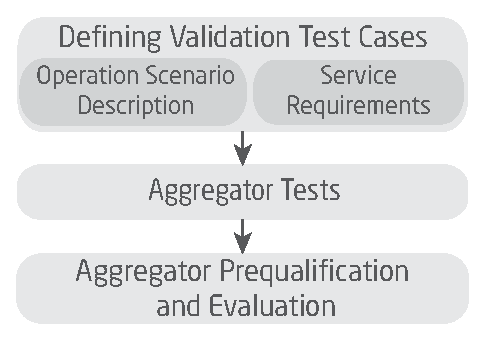
\includegraphics[width=0.7\textwidth]{validationMAIN.eps}
\caption{Schematic process for aggregator validation.}
\label{fig:MAINframework}
\end{figure}

\begin{figure}[htpb!]
\centering
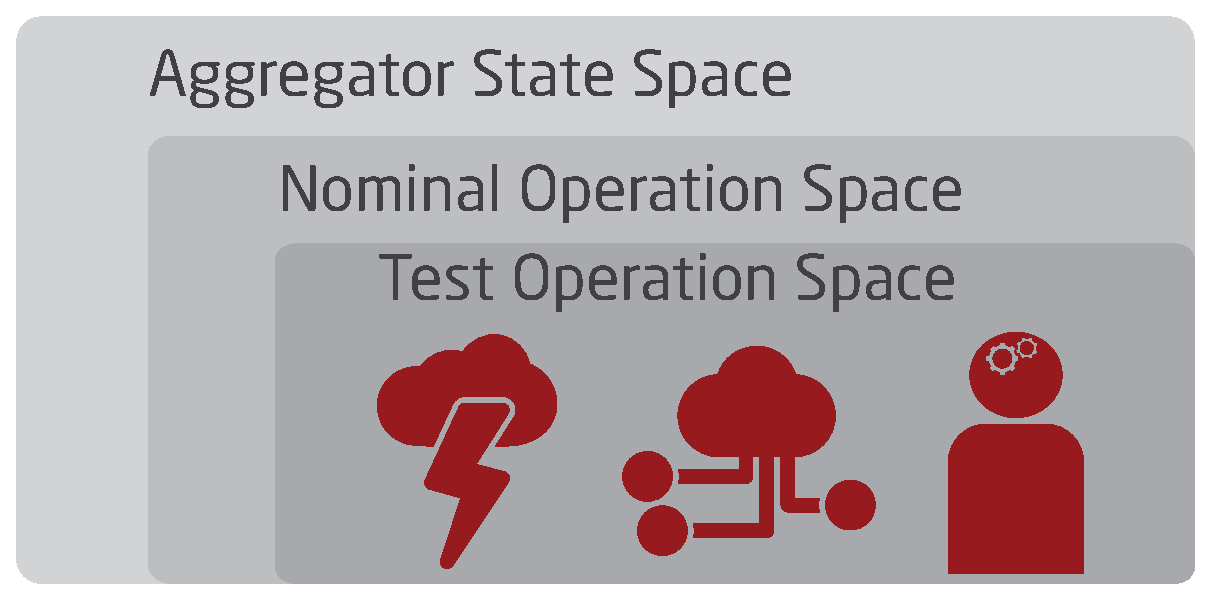
\includegraphics[width=0.8\textwidth]{aggstatespace.eps}
\caption{From all the possible state space the aggregator can operate in, it is only a subset that is considered nominal operation. Within this nominal operation, a test operation space is defined, where the stochastic variables that affect the aggregator performance are manipulated to test the aggregator reliability. These stochastic variables include, but are not limited to, weather conditions, communication failure and user behavior.}
\label{fig:aggstatespace}
\end{figure}

The proposed simulation tests should be carried out within a validation framework, as depicted in Figure~\ref{fig:frameworkbig}. The service requirements describe the goal the aggregator needs to achieve and the test scenarios define the normal operation disturbances that an aggregator should handle. The aggregator will not be held responsible for service non-delivery when it is affected by major problems outside it responsibility domain, e.g. in case of severe grid faults. The service requirements are discussed in depth in Chapter~\ref{cha:services} and the service verification and evaluation is discussed in depth in Chapter~\ref{cha:verification}.

\begin{figure}[ht]
	\centering
	\caption{The validation framework, where the aggregator is the unit-to-test, is ideally composed of a software co-simulation platform with hardware-in-the-loop capabilities. The inputs are the validation test cases, and the output (i.e. the service) is verified and evaluated. The arrows represent information exchange.}
	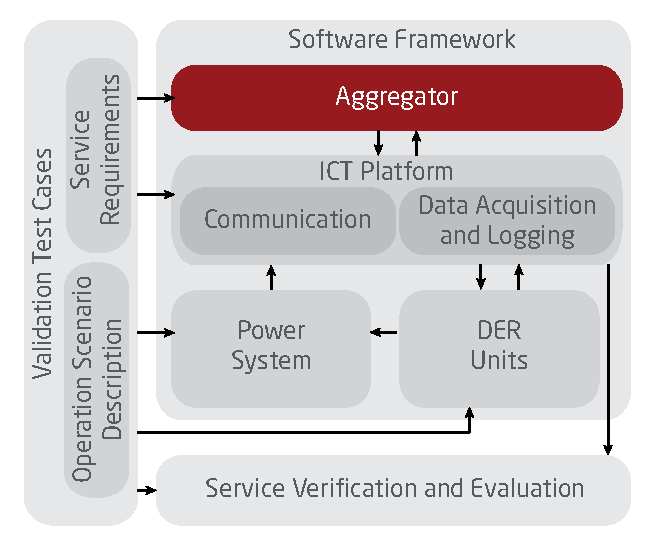
\includegraphics[width=\textwidth]{framework/framework.eps}\label{fig:frameworkbig}
\end{figure}

\section{Service Requirements and Test Alignment} 
\newsection{F}{rom the previous} section it is clear that the service requirements form an essential part of the aggregator validation process. Service requirements are discussed in the depth in Chapter~\ref{cha:services}, but a set of test service requirement metrics have been formulated as part of the test method and are presented here.

In order to measure how disturbances\footnote{See Figure~\ref{sec:servreqmet} for a visual representation of how disturbances affect the aggregator} affect service delivery, a set of performance metrics must defined. Based upon the current ancillary service definition, the chosen metrics are:
\begin{description}
	\item[Time responsiveness:] how fast can the service be delivered from the moment the reference or measurement signal changes.
	\item[Grid responsiveness:] how well can the aggregator follow changes in the grid state.
	\item[Response accuracy:] how good is the aggregator at providing the full volume that is requested.
\end{description}

It is the TSO that defines the value of these metrics that signify a passed validation test. Since the tests are stochastic, the metric value should also have a stochastic component, this could for example be \emph{time responsiveness} of service provision of 5 seconds with variance of $\pm$ 1 second. The metrics must be measured by an index and while literature has a wide array of indices for measuring performance, a specific index for aggregators is presented in Chapter~\ref{cha:verification}.

In order to align the service requirements and the test design, the following steps are proposed:
\begin{enumerate}
	\item The aggregator informs of the general composition of its portfolio, as well as the service it wants to be validated for.
	\item The tester identifies the appropriate service requirements for the service to be tested for.
	\item The tester identifies the expected normal operation of the aggregator.
	\item The tester defines the test operation scenarios that the aggregator is expected to perform under. The scenarios must define the statistical properties, e.g. mean and variance, for the stochastic disturbances affecting the aggregator performance.
	\item The tests are carried out on the aggregator.
	\item The aggregator performance is evaluated.	
\end{enumerate}

Note that the entity performing the validation tests can be an independent party, e.g. a third party certifier for aggregators, or it can be the TSO.

Depending on the excitation signals the aggregator is subject to, the tests are divided into two categories:
\begin{itemize}
	\item step response, and
	\item continuous reference tracking.
\end{itemize}
The kind of test used for the validation will depend on the test scenario description.

\section{Short on Prequalification of Aggregators}
\newsection{I}{t was previously mentioned} that traditional generator prequalification consists of two steps, the documentation of the generator and the response test. In Chapter~\ref{cha:aggregator} a functional reference framework for aggregators was introduced. This reference architecture can be used as a checklist, along with the test results from the validation framework as the documentation part of the prequalification of aggregators. A response test should be performed, not to validate the aggregator reliability, but to verify the communication between the TSO control center and the aggregator. Furthermore, aggregator performance should be continually evaluated, and new validation tests should be carried out routinely. This is due to the dynamic nature of the aggregator portfolio, which may regularly change in size and composition.

\section{Conclusions Regarding the Validation Framework}
\newsection{T}{he concept of validation} of aggregators is important for the participation of aggregators in both ancillary services markets and energy markets. The original contribution of this work is the design of the aggregator validation framework and specially the analysis of aligning service requirements with test design. The described approach to test the system through statistical methods and define the requirements as with statistical values is novel.

A weakness in the proposed method is that the validation tests are highly dependable on the accuracy of the used models in the simulation. A way to mitigate this is to make the framework modular so that the tests can be run with hardware-in-the-loop (for model validation of individual units) or so that the framework can be connected to validated models, e.g. a Real-Time Digital Simulator (RTDS). 

Future work will consist of further refining the validation architecture, specifically defining the interfaces between modules, and implementing the software platform.
